\subsection{Gateway}
	Un \textit{gateway} è una componente localizzata all'interno di un'azienda che permette di rendere uniforme l'interfaccia di accesso ai dati dei singoli dispositivi configurati all'interno del gateway stesso.
	\newline
	Dai gateway è possibile inoltre configurare funzioni di accumulo dei pacchetti contenenti i dati dei sensori o di impostare alcuni timer, al termine dei quali deve essere effettuato l'invio dei dati all'interno dei rispettivi topic di \glock{Kafka}.
	\newline
	Tutte le configurazioni vengono ricevute tramite appositi topic adibiti esclusivamente a questa funzione.
	\begin{itemize}
		\item La componente è stata sviluppata in Java 11.
	\end{itemize}
	
	\subsubsection{Diagramma dei package}%%%%%%%%%%%%OK
	  	\begin{figure}[H]
			\centering
			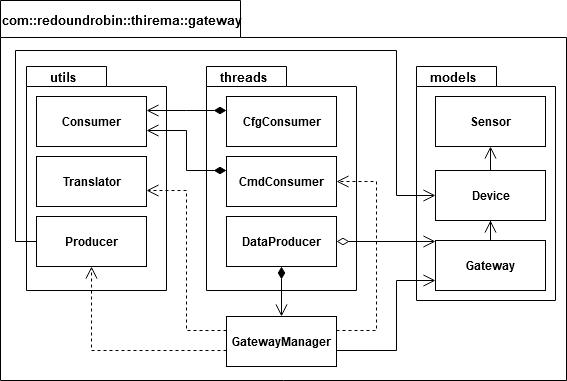
\includegraphics[scale=0.550]{res/images/GATEWAY/GatewayPackage.png}
			\caption{Diagramma dei package per la componente gateway}
			\label{Diagramma 1}
		\end{figure}
	\subsubsection{Dipendenze esterne}	
		La componente gateway ha due dipendenze esterne: 
			\begin{itemize}
				\item \textbf{KafkaProducer<K, V>}, classe concreta che implementa l'interfaccia Producer<K,V>. Svolge il compito di client per il cluster \glock{Kafka}, pubblicando dati all'interno di un topic. La classe Producer ne possiede un riferimento.
				\item \textbf{KafkaConsumer<K,V>}, classe concreta che implementa l'interfaccia Consumer<K,V>. Svolge il compito di client per il cluster \glock{Kafka}, consumando i messaggi resenti all'interno di uno o più topic. La classe Consumer ne possiede un riferimento.
			\end{itemize}	
		\newpage		

	\begin{landscape}
		\subsubsection{Diagramma delle classi}%%%%%%%%%%%%%%%%%%%%%%%OK
		  	\begin{figure}[H]
				\centering
				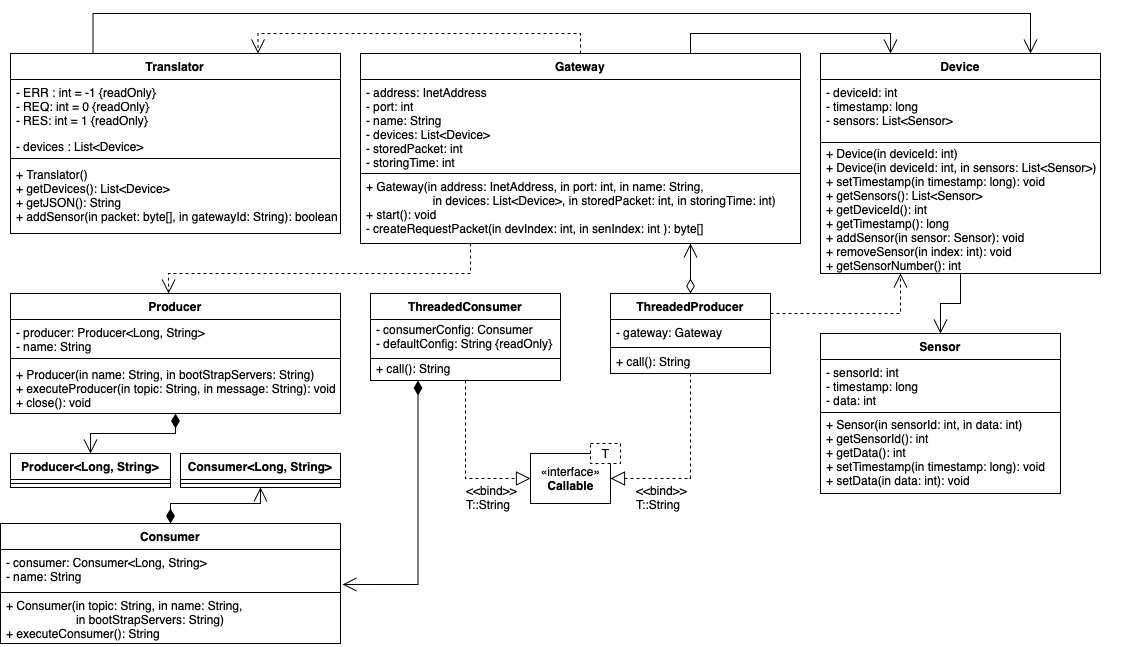
\includegraphics[scale=0.499]{res/images/GATEWAY/ClassiGateway.png}
				\caption{Diagramma delle classi per la componente gateway}
				\label{Diagramma 2}
			\end{figure}
	Come si evince dal diagramma sono presenti le seguenti classi:
	\begin{itemize}
		\item \textbf{Consumer}: rappresenta un consumer di Kafka, che è infatti contenuto al suo interno. La classe viene utilizzata per "consumare" messaggi da uno o più topic di Kafka (in questo caso dal topic delle configurazioni); 
		\item \textbf{Producer}: rappresenta un producer di Kafka, che è infatti contenuto al suo interno. La classe viene utilizzata per "produrre" messaggi contenenti le rilevazioni del valori dei sensori all'interno di un topic Kafka;
		\item \textbf{ThreadedConsumer}: classe che contiene al suo interno un Consumer per poter reperire da un topic \glock{Kafka} le configurazioni per il gateway. Appena ne riceve una, viene sostituita alla vecchia configurazione e viene ripresa l'attività di fetching dei dati;
		\item \textbf{ThreadedProducer}: classe che contiene un riferimento a Gateway, in cui si trova la business logic per la richiesta al simulatore e l'invio dei dati a Kafka. Per poter fare ciò necessita della classe Translator per convertire i dati in JSON e delle classi Device e Sensor per costruire la lista di dispositivi a cui dovrà richiedere i dati;
		\item \textbf{GatewayManager}: classe che contiene buona parte della logica della componente Gateway: al suo interno infatti è presente un ciclo che itera tutti i dispositivi di tutti i sensori richiedendo ad ognuno dei dati. Quando ne raccoglie un certo numero o passano n secondi (in base alla configurazione del gateway) questi dati vengono inviati ad un topic ed il ciclo si ripete;
		\item \textbf{Translator}:classe che, come detto brevemente in precedenza, viene utilizzata per accumulare e tradurre ciò che viene restituito dai sensori in un pacchetto in formato JSON che poi verrà inviato in un topic;
		\item \textbf{Gateway}: rappresenta il gateway; è infatti presente un identificativo (name), una lista di device (devices) e l'indirizzo (address) e la porta (port) a cui inviare le richieste dei dati dei dispositivi;
		\item \textbf{Sensor}: rappresenta il dato di un singolo sensore; è infatti presente un identificativo (sensorId), un valore (data) ed infine il timestamp legato a quando è stata fatta la rilevazione del valore;
		\item \textbf{Device}: rappresenta un dispositivo; al suo interno è presente una lista di Sensor (sensors), un identificativo (deviceId) ed un timestamp legato a quando è stata fatta l'ultima rilevazione di uno qualsiasi dei suoi sensori.
	\end{itemize}
	\end{landscape}
		
	\begin{landscape}
		\subsubsection{Diagramma di sequenza}%%%%%%%%%%%%%%%%%%%%%%%OK
		  	\begin{figure}[H]
				\centering
				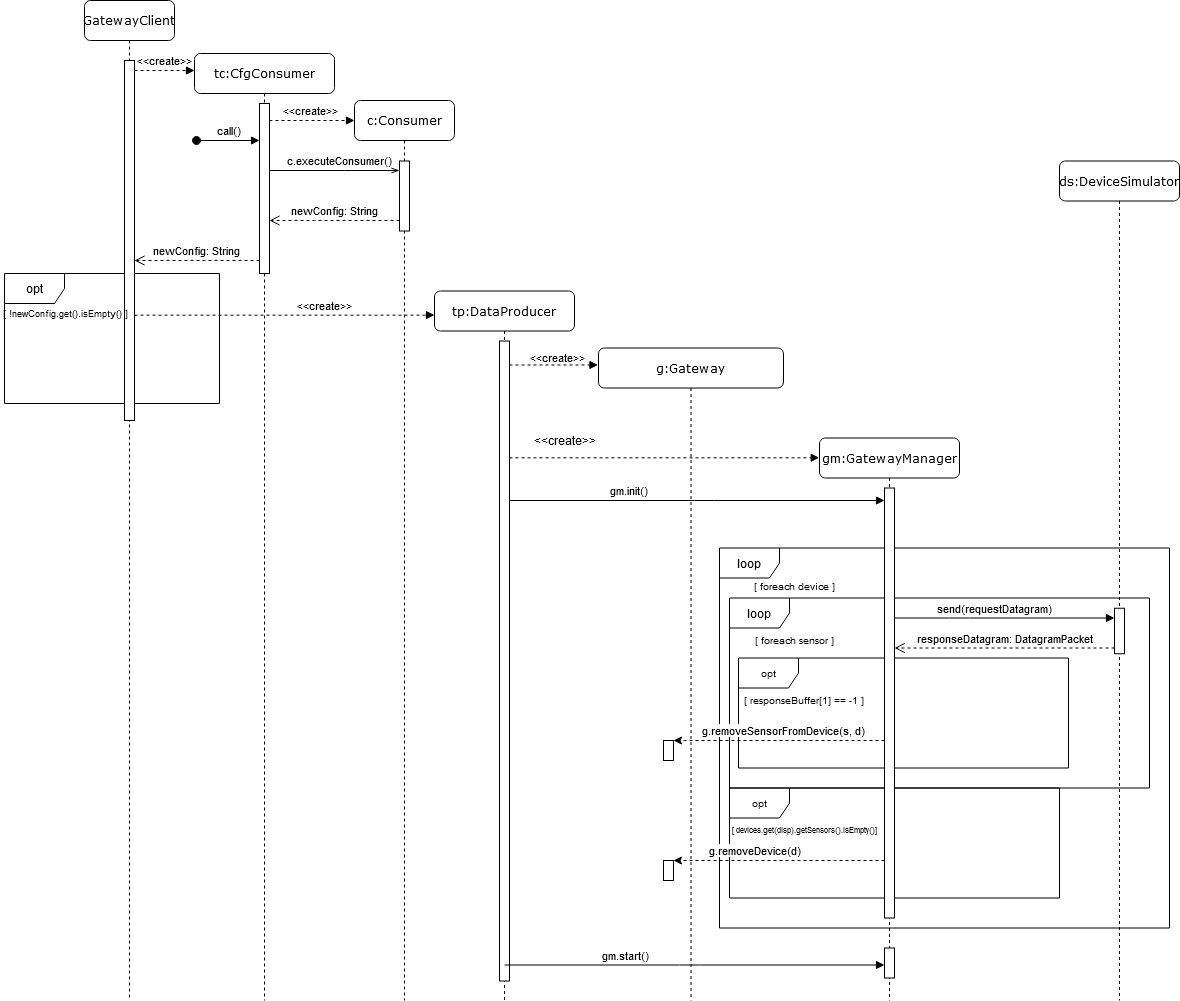
\includegraphics[scale=0.400]{res/images/GATEWAY/RichiestaInvioGateway.png}
				\caption{Diagramma di sequenza che rappresenta la richiesta di una prima configurazione ed un primo settaggio del gateway}
				\label{Diagramma 3}
			\end{figure}
			Nel diagramma di sequenza è rappresentata la richiesta e la ricezione di una prima configurazione da parte del ThreadedConsumer.
			\newline
			La configurazione viene quindi passata al ThreadedProducer, che tramite un metodo crea il Gateway e il GatewayManager (sulla base della configurazione ottenuta) e questo, tramite il metodo init() verifica che tutti i dispositivi nella configurazione siano effettivamente presenti.
	\end{landscape}
	
	\subsubsection{Diagramma di attività}%%%%%%%%%%%%%%OK
		\begin{figure}[H]
			\centering
			\includegraphics[scale=0.500]{res/images/GATEWAY/gateway.start().png}
			\caption{Diagramma di attività che rappresenta un'iterazione all'interno del metodo start() della classe gateway}
			\label{Diagramma 4}
		\end{figure}
		 Nel diagramma è rappresentato il metodo start() della classe Gateway, in cui vengono creati dei pacchetti di richiesta e vengono inviati al simulatore dei dispositivi.
		 \newline
		 Quest'ultimo, dopo aver generato i dati, invia un pacchetto di risposta che, se è integro, viene aggiunto ad un buffer che, una volta pieno, viene inviato ad un topic \glock{Kafka}.   
		